\documentclass[10pt,a4paper]{article}
\usepackage[utf8]{inputenc}
\usepackage[basque]{babel}
\usepackage{amsmath}
\usepackage{amsfonts}
\usepackage{amssymb}
\usepackage{makeidx}
\usepackage{graphicx}
\graphicspath{ {images/} }
\usepackage{lmodern}
\usepackage[left=3cm,right=3cm,top=3cm,bottom=2cm]{geometry}
\usepackage{fancyhdr}
\usepackage{montserrat}
\usepackage{lastpage}
\usepackage{afterpage}
\newcommand\blankpage{%
	\null
	\thispagestyle{empty}%
    \addtocounter{page}{-1}%
	\newpage}

\usepackage[export]{adjustbox}
\usepackage{wrapfig}
\usepackage{hyperref}

\usepackage{nameref}

\setlength\parindent{0pt}

\usepackage{xcolor}
\usepackage{titlesec}
  
\let\nf\normalfont %\nf komandoari \nf deitu  
\newcommand{\cf}{\normalfont\sffamily}

  
\titleformat{\section}
  {\nf\sffamily\Large}
  {\thesection}{1em}{}

\titleformat{\subsection}
  {\nf\sffamily\Large}
  {\thesubsection}{1em}{}

\renewcommand{\footrulewidth}{0pt}

\pagestyle{fancy}
\fancyhf{}
\lhead{\cf 2019/09/21}
\chead{\cf v 1.1}
\rhead{\cf \# 411-000}
\fancyfoot[C]{\cf\thepage /\pageref{LastPage}}


\title{\cf \# 411-000 \\ \vspace{5mm}
					Product Breakdown Structure (PBS) sistema baten erabilera MinervaLab-en garapenean \\
\normalsize \vspace{5mm} Data: 2019/09/21 \\
 			\vspace{3mm} Bertsioa: 1.1}
\date{}
%\author{Jon Gabirondo López}

\begin{document}

\maketitle
\thispagestyle{fancy}
%\author

\section{Hasierako egoera}
MinervaLab proiektuaren helburua Termodinamika eta Fisika Estatistikoaren inguruko grafika interaktiboen sorta bat garatzea da. Landu daitezkeen gai zein kontzeptuen ugaritasuna eta konplexutasunari erreparatuz, amaierako programa luzea eta nahiko heterogeneoa izatea aurreikusi daiteke. Honegatik, MinervaLab osatuko duten programa txikien garapena elkarren artean ahalik eta independenteki eta paraleloki egin ahal izateko planteatu nahi da. Gainera, programazio denborak murriztu eta optimizatzea ere beharrezkoa izango da proiektua garaiz amaitu ahal izateko.
\\

Honegatik, MinervaLab-en garapena kudeatzeko PBS sistema bat planteatzen da. 

\section{Helburua}
Erabiliko den PBS sistemak hainbat helburu ditu:
\begin{itemize}
\item Programa txikien edota kode 'zelula' guztien egoeraren berri eramatea.
\item Programatze-saio ororen aurretik idatzi beharreko programaren inguruko hausnarketa egotea, textu liburu edota beste iturrietan oinarrituta.
\item  Programatzen hasi aurretik egin beharrekoaren txosten bat izatea, proiektuko zuzendariak aurretik zuzendutakoa.
\item Garapenean proiektuko taldekideek (zuzendaria eta garatzailea, kasu honetan) independenteki lan egin ahal izatea, bakoitza atal ezberdinetan zentratuz.
\end{itemize}

 
\section{Garapena}
PBS sistema aurrera eramateko bi elementu nagusi behar dira: proiektuaren egoera jasoko duen \textbf{taula bat} eta programen \textbf{txostenak}.
\\

\newpage

Aipatutako taulak honelako itxura izango du:

\begin{figure}[h]
\centering
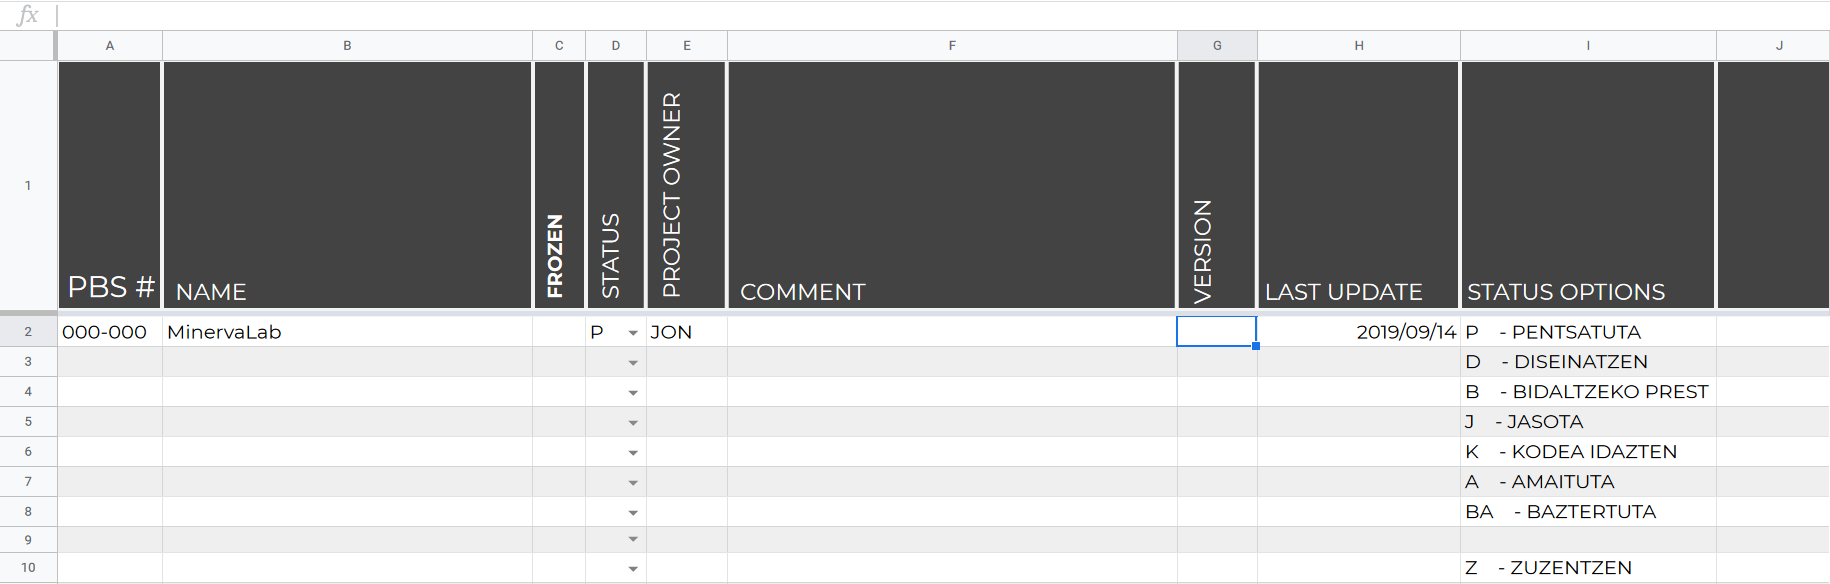
\includegraphics[width=\linewidth]{1}
\caption{PBSaren taularen konfigurazio posible bat.}
\end{figure}

Hauek dira taulan aurkitu daitezkeen zutabeak:

\begin{enumerate}
\item \cf PBS \#: \nf Elementu horri dagokion kodea. 
\\

Kodea 0 eta F bitarteko 6 digito alfanumerikoez osatuta egongo da. Lehenengo hiru digitoek programa nagusiari erreferentzia egingo diote eta azken hirurek programa nagusiaren azpiatal bakoitzari.
\\

\begin{center}
\cf \# ABC-DEF
\end{center}

\cf A \nf digitoak zein elementu mota den adieraziko du:


\begin{table}[h]
\begin{center}
\begin{tabular}{|c|c|}
\hline
\textbf{Zenbakia} & \textbf{Elementua} \\ \hline
0                 & MinervaLab         \\ \hline
1                 & Kodea              \\ \hline
2                 & Dokumentazioa      \\ \hline
3                 & Txostena           \\ \hline
4                 & Bestelakoak           \\ \hline
\end{tabular}
\caption{\cf A \nf digitoaren kodeketa}
\end{center}
\end{table}

\cf B \nf digitoak elementuak landu beharreko gaia adieraziko du. Adibidez, Van der Waals-en ekuazioaren inguruko programek \cf \# 11X-000 \nf kodea izango lukete.
\\

\cf C \nf digitoak \cf B \nf digitoak adierazitako gaiaren inguruko programa ezberdinak adieraziko ditu. Adibidez, Van der Waals-en ekuazioa 2Dtan lantzen dituen programak \cf \# 111-000 \nf kodea izan dezake eta 3Dtan lantzen dituen programak \cf \# 112-000 \nf kodea izan dezake.
\\

Azken hiru digitoek lehenengo hirurek adierazitako elementuaren azpiatalak adieraziko dituzte, ordenean.
\\

Programatzen hasi aurretik sortutako txostenak hemen azaldutako kodeketan oinarrituko dira programaren helburu eta nondik norakoak azaltzeko.
\\

Erreparatu sistema hau erabiliz programa baten kodearen eta bere dokumentazioaren kodearen arteko diferentzia lehenengo digitoa baino ez dela izango.
\\ 

\item \cf NAME: \nf Elementuaren izena.
\\

\item \cf FROZEN: \nf 'BAI' ala 'EZ' izan daiteke, elementu hori aktiboki garatzen ari den ala ez adierazteko.
\\

\item \cf STATUS: \nf Elementuaren egoerari buruzko informazioa gordetzen du eta \cf STATUS OPTIONS \nf zutabean ikus daitezkeen aukeretako bat izango da.
\\

\item \cf PROYECT OWNER: \nf Une horretan elementuan lan egiten ari den pertsona adierazten du. Elementu baten \cf STATUS \nf zutabearen balioa \cf 'Z - ZUZENTZEN' \nf bada, zuzentzailearen izena agertuko da, bestela, garatzailearena.
\\

\item \cf COMMENT: \nf Elementuaren inguruko iruzkin bat.
\\

\item \cf VERSION: \nf Elementuaren bertsioa.
\\

\item \cf LAST UPDATE: \nf Elementuaren egoera azkenengo aldiz aldatu zenenko data.
\\
\end{enumerate} 

\section{Lan-fluxua}

Elementu bat garatzean \cf STATUS OPTIONS \nf eko etapa ezberdinetatik igarotzen joango da, aurreko egoera batera itzultzeko aukera izango duelarik (berrikusketa bat egitean edo).
 
\begin{thebibliography}{1}
\bibitem{1} Molin, M. [Wintergatan]. (2018, urriak 18). \textit{How to Organize Your Project with a PBS System - Marble Machine X \# 57} [Video file]. Retrieved from \url{https://www.youtube.com/watch?v=zVyEsMiwvVc&t=512s}.
\end{thebibliography}

\end{document}